\documentclass[11pt, a4paper]{article}
\usepackage[a4paper, margin=1in]{geometry}


\usepackage{adjustbox}
\usepackage{mathtools}
\usepackage{amsmath}
\usepackage{amssymb}
\usepackage{amsthm}

\usepackage{pgfplots}
\usepackage{listings}
\usepackage{color}
\usepackage{tikz}

\usepackage{textcomp}
\usepackage{soul}

\usepackage[hidelinks]{hyperref}
\pgfplotsset{width=7.5cm,compat=1.12}
\usepgfplotslibrary{fillbetween}
\usepackage[makeroom]{cancel}
\title{\bf{Homework \textnumero 1}}
\author{Author: David Oniani
\\
\ \ \ Instructor: Dr. Eric Westlund}
\date{February 9, 2019}

\usepackage{listings}
\usepackage{color}

%%%%%%%%%%%%%%% S E T S %%%%%%%%%%%%%%%
\newcommand{\nats}{\mathbb{N}}
\newcommand{\ints}{\mathbb{Z}}
\newcommand{\rats}{\mathbb{Q}}
\newcommand{\reals}{\mathbb{R}}
\newcommand{\irrats}{\mathbb{I}}

\newcommand{\pnats}{\mathbb{N}^+}
\newcommand{\pints}{\mathbb{Z}^+}
\newcommand{\prats}{\mathbb{Q}^+}
\newcommand{\preals}{\mathbb{R}^+}
\newcommand{\nreals}{\mathbb{R}^-}

\newcommand{\nints}{\mathbb{Z}^-}
\newcommand{\nrats}{\mathbb{Q}^-}
%%%%%%%%%%%%%%%%%%%%%%%%%%%%%%%%%%%%%%%

% Calligraphy
\newcommand\und[1]{\underline{\smash{#1}}}

% Operators
\DeclarePairedDelimiter\abs{\lvert}{\rvert}
\DeclarePairedDelimiter\ceil{\lceil}{\rceil}
\DeclarePairedDelimiter\floor{\lfloor}{\rfloor}

% Other
\newcommand{\rarr}{\rightarrow}

\definecolor{dkgreen}{rgb}{0,0.6,0}
\definecolor{gray}{rgb}{0.5,0.5,0.5}
\definecolor{mauve}{rgb}{0.58,0,0.82}
\definecolor{backcolour}{rgb}{0.95,0.95,0.92}

\lstset{
backgroundcolor=\color{backcolour},
aboveskip=3mm,
belowskip=3mm,
showstringspaces=false,
columns=flexible,
basicstyle={\small\ttfamily},
numbers=left,
numberstyle=\normalsize\color{gray},
keywordstyle=\color{blue},
commentstyle=\color{dkgreen},
stringstyle=\color{mauve},
breaklines=true,
breakatwhitespace=true,
tabsize=4
}


\begin{document}
\maketitle
\begin{itemize}
\item[1.6]
Since the max percentage is 27.1, we will have 6 bars.
Notice that we have:
\begin{align*}
&19 \mbox{ states in the category from } 0\% \mbox{ to } < 5.0\%\\
&16 \mbox{ states in the category from } 5.0\% \mbox{ to } < 10.0\%\\
&9 \mbox{ states in the category from } 10.0\% \mbox{ to } < 15.0\%\\
&3 \mbox{ states in the category from } 15.0\% \mbox{ to } < 20.0\%\\
&2 \mbox{ states in the category from } 20.0\% \mbox{ to } < 25.0\%\\
&1 \mbox{ state in the category from } 25.0\% \mbox{ to } < 30.0\%\\
\end{align*}

Also, notice that $19 + 16 + 9 + 3 + 2 + 1 = 50$ (so hope I did not miscategorize any state).
Then the histogram for this data will be:

\begin{center}
    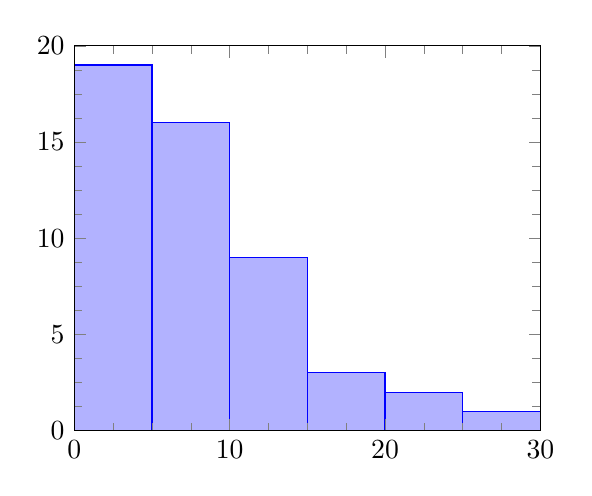
\begin{tikzpicture}
        \begin{axis}[
            ymin=0, ymax=20,
            xmin=0, xmax=30,
            minor y tick num = 3,
            minor x tick num = 3,
            area style,
            ]
        \addplot+[ybar interval, mark=no] plot coordinates { (0, 19) (5, 16) (10, 9) (15, 3) (20, 2) (25, 1) (30, 1) };
        \end{axis}
    \end{tikzpicture}
\end{center}

\item[]
\item[]

\item[1.8]
It is easy to see that the distribution is skewed and not symmetric.
Particularly, this is the right-skewed distribution since its tail is to the right.
The midpoint seems to be $15$. The percent of state population born outside the united
states ranges from $1.3\%$ to $27.1\%$, which shows considerable variability.
There are no states with unusually large or small percent of foreign-born residents
since there are no gaps in the histogram.

\item[]
\item[]
\item[]

\item[1.10]
\begin{itemize}
\item[(a)]
The stemplot will look like this:

\item[]
\item[]
\begin{tabular}{r | *{120}{c}}
    5 & 9\\
    6 & 2 & 3 & 7 & 8 & 8\\
    7 & 1 & 1 & 2 & 4 & 4 & 4 & 5 & 6 & 6 & 6 & 6 & 7 & 7 & 7 & 8 & 8 & 8\\
    8 & 0 & 0 & 0 & 1 & 1 & 2 & 2 & 3 & 3 & 3 & 3 & 3 & 3 & 3 & 4 & 4 & 6 & 6 & 6 & 6 & 6 & 6 & 7 & 7 & 8
\end{tabular}
\item[]
\item[]

From this stemplot, it is easy to see that the midpoint is $80$ and that the variability
is from $59\%$ to $88\%$.

\item[]

\item[(b)]
The stemplot will look like this:

\item[]
\item[]
\begin{tabular}{r | *{120}{c}}
    5 &\\
    5 & 9\\
    6 & 2 & 3\\
    6 & 7 & 8 & 8\\
    7 & 1 & 1 & 2 & 4 & 4 & 4\\
    7 & 5 & 6 & 6 & 6 & 6 & 7 & 7 & 7 & 8 & 8 & 8\\
    8 & 0 & 0 & 0 & 1 & 1 & 2 & 2 & 3 & 3 & 3 & 3 & 3 & 3 & 3 & 4 & 4\\
    8 & 6 & 6 & 6 & 6 & 6 & 6 & 7 & 7 & 8
\end{tabular}
\item[]
\item[]

In this stemplot, the shape of the distribution is a lot clearer (compared to histogram in Figure 1.5) to see.
Though, it actually does give us a histogram if we put bars on top of these numbers.
\end{itemize}

\item[]
\item[]

\item[1.12]
\item[(a)]
\begin{itemize}
The time plot will look like this:

\item[]
\item[]
\item[]
\begin{center}
    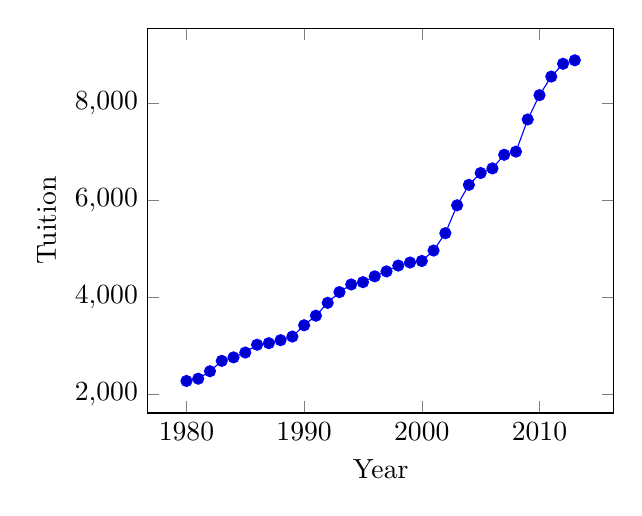
\begin{tikzpicture}
        \begin{axis}[
            xlabel=Year,
            ylabel=Tuition,
            % remove comma in xticklabels
            xticklabel style={/pgf/number format/set thousands separator={}},
            % one tick every 10 years
            xtick distance=10
            ]
            \addplot table {
            Year Tuition
            1980 2274
            1981 2321
            1982 2475
            1983 2689
            1984 2761
            1985 2861
            1986 3022
            1987 3054
            1988 3116
            1989 3191
            1990 3424
            1991 3621
            1992 3887
            1993 4108
            1994 4266
            1995 4314
            1996 4434
            1997 4536
            1998 4656
            1999 4719
            2000 4751
            2001 4966
            2002 5324
            2003 5900
            2004 6322
            2005 6566
            2006 6662
            2007 6943
            2008 7008
            2009 7672
            2010 8174
            2011 8557
            2012 8821
            2013 8893
            };
            % if you have the file, you can do
            % \addplot table {datafile.csv};
        \end{axis}
    \end{tikzpicture}
\end{center}

\item[(b)]
The overall pattern is that over the years, the tuition increases.

\item[]

\item[(c)]
From 2001 to 2004 and from 2009 to 2012, we have periods of rapid increase.\\
No other deviations are present.

\item[]

\item[(d)]
The percent increase would be better. Because it would also show us the how the change over time itself changes.
\end{itemize}

\item[]
\item[]

\item[1.27]
\begin{itemize}
\item[(a)]
The bar chart will look like this:

\begin{center}
    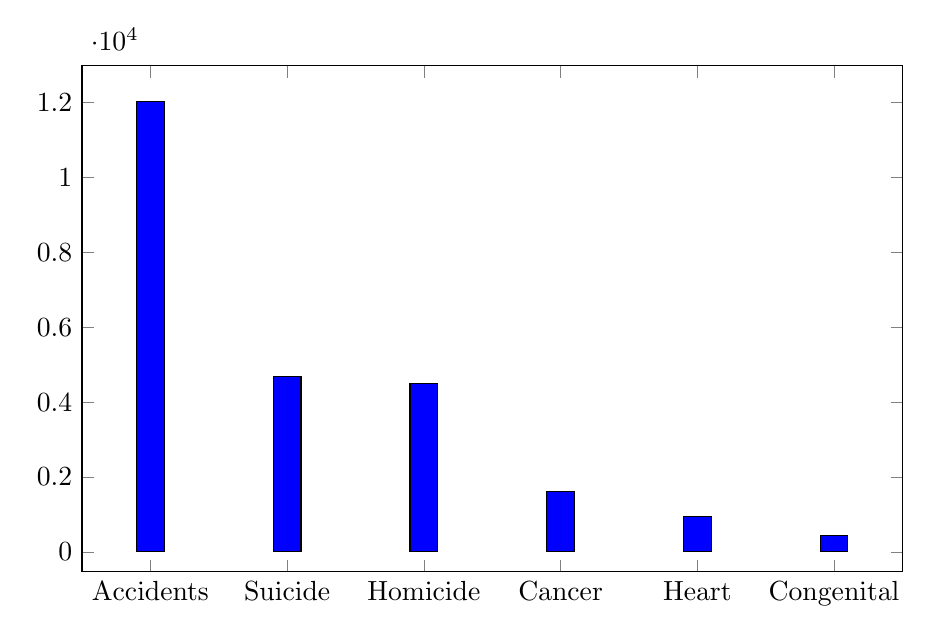
\begin{tikzpicture}
        \begin{axis}[
            symbolic x coords={Accidents, Suicide, Homicide, Cancer, Heart, Congenital},
            xtick=data,
            height=8cm,
            width=12cm,
            enlarge y limits={abs=0.45cm}
          ]
            \addplot[ybar,fill=blue] coordinates {
                (Accidents, 12032)
                (Suicide, 4688)
                (Homicide, 4508)
                (Cancer, 1609)
                (Heart, 948)
                (Congenital, 429)
            };
        \end{axis}
    \end{tikzpicture}
\end{center}

Notice that $0, 0.2, 0.4, 0.6, 0.8, 1, 1.2$ are all times $10^4$.

\item[]

\item[(b)]
We would need to know how many people died from other causes since one cannot
construct a pie chart without knowing what is the ``whole picture.''
\end{itemize}

\item[]
\item[]

\item[1.28]
They come from Mexico, Puerto Rico, Cuba, Central America, South America, and other regions.
If my eyeballs tell the truth, then Mexicans must be somewhere around $60\%$ ($\frac{3}{5}$ of the pie) of Hispanics.
And approximately $10\%$ ($\frac{1}{10}$ of the pie) of Hispanics are Puerto Rican.

\item[]
\item[]

\item[1.33]
\begin{itemize}
\item[2.]
Are you right-handed or left-handed? -- This would go with graph (b)
since, generally speaking, there are more right-handed people than left-handed ones.

\item[1.]
Are you female or male? -- This would go with graph (c). This is due to elimination.
If it is not graph (b), it must be graph (c) since being a male or female is a binary option
and all other graphs have more than $2$ bars.

\item[3.]
What is your height in inches? -- The graph must look sort of symmetric since, generally speaking,
there always is a great diversity in height (some are tall, some are average, some are short). The only
symmetrically-looking graph is (d). Therefore, graph (d) seems to be the best option here.

\item[4.]
How many minutes do you study on a typical weeknight? -- Due to the elimination, we are left with the
graph (a) which indeed makes sense since not a lot of people will study for a very long time
resulting in the right-skewed distribution.
\end{itemize}

\item[]
\item[]

\item[1.36]
\begin{itemize}
\item[(a)]
A country with the bigger population would have a bigger CO$_2$ emission rate.

\item[]

\item[(b)]
I will round it to the nearest tenth (although rounding it to the nearest hundredth/thousandth/etc. is more precise,
it is super inconvenient and a lot of work too). This is how the stemplot looks like:

\item[]
\item[]
\begin{tabular}{r | *{120}{c}}
    0 & 1 & 1 & 2 & 2 & 3 & 3 & 4 & 5 & 5 & 9 & 9\\
    1 & 6 & 6 & 7 & 7 & 8\\
    2 & 2 & 6\\
    3 & 3 & 7 & 8\\
    4 & 4\\
    5 & 6 & 9\\
    6 & 2 & 6 & 7\\
    7 & 7 & 9\\
    8 & 3\\
    9 & 1 & 2 & 2\\
    10 &\\
    11 & 5\\
    12 & 2\\
    13 &\\
    14 & 6\\
    15 &\\
    16 &\\
    17 & 6\\
\end{tabular}
\item[]
\item[]
where $0 \mid 1 = 0.1$, $2 \mid 6 = 2.6$ etc.
\item[]
\item[]

It is easy to see that the distribution is right-skewed.
The center will be at $2$ (there are $37$ datapoints in total and the $18^{\text{th}}$ is $26$).
Variability is from $0.1$ to $17.6$. The US ($17.6$) and Canada ($14.6$) are the outliers.
\end{itemize}

\newpage

\item[1.38]
\begin{itemize}
\item[(a)]
They mean that there were no improvements at all and that the task completion time worsened.

\item[]

\item[(b)]
The back-to-back stemplot looks like this:
\item[]
\item[]
\begin{tabular}{r | *{1}{c} | *{1}{c}}
    Treatment & & Control\\
     & -0 & 8\\
    1 2 2 & -0 & 3 1\\
     & 0 & 5 5 6 7 7 8 9 9 9 9\\
    8 8 8 7 7 6 & 0 & 2 3 3 4 4\\
    4 3 3 3 2 & 1 & 5\\
    8 & 1 & 1\\
    4 4 2 1 & 2 & 3\\
    8 & 2 & 3\\
    3 & 3 &\\
\end{tabular}
\item[]
\item[]
Note that numbers like 85 are rounded to 90. In other words, anything that ends with 0, 1, 2, 3, 4
gets rounded DOWN  to 0 and anything that ends with 5, 6, 7, 8, 9 is rounded UP to 0.
\item[]
\item[]

\item[(c)]
The midpoint for treatment is $130$ and the midpoint for control is $90$.
No, it does not seem so. This is since $130 > 90$. Hence, control group did better.
This is still somewhat inaccurate estimate since the problem gives us a median
without saying whether the previous distribution was skewed or symmetric.
\end{itemize}
\item[]
\item[]

\item[1.43]
\begin{itemize}
\item[(a)]
Graph (a). In other words, if we drew an approximation lines for both graphs,
then the slope of the line for graph (a) would be bigger than that for graph (b).

\item[]

\item[(b)]
The increase in tuition from $2000$ to $2013$ seems to be the same for both graphs.
It is approximately $\$6, 000$. I think that the graphs are for the same dataset,
it is just the scaling on the vertical axis that is different.

\end{itemize}
\end{itemize}
\end{document}
